\chapter{Introduction}\label{ch:introduction}
\markboth{}{Introduction}
\addcontentsline{toc}{chapter}{Introduction}

\todo{for some reason in the TOC the chapter name appears twice. Is that intentional?}
\todo{What is the thesis about? What is the content of it? What is the Author's contribution to it?}
\todo{I used game and thesis and program and application and work interchangeably. We should define these terms and use them accordingly.}

The main goal of this thesis is to create a video game that combines the concepts of procedural generation and non-Euclidean geometry.
Procedural generation is a method used to create the world by using algorithms instead of manually designing it.
It was first used in the 1980s in games such as \textit{Elite} \cite{Elite1984} and \textit{Rogue} \cite{Rogue1980} and has achieved a significant increase in popularity with the release of \textit{Minecraft} \cite{Minecraft} in 2011.
Unlike procedural generation, which has a long and rich history in the video game industry, the concept of employing non-Euclidean geometries is a relatively novel idea.
It has been used in only a few games, most notably in \textit{Hyperbolica} \cite{Hyperbolica}, which was released in 2022.
Non-Euclidean geometry differs from the usual Euclidean geometry in that it does not satisfy the parallel postulate -- one of the postulates given by Euclid.
This postulate states that given a line and a point not on the line, there is exactly one line through the point that does not intersect the given line.
In non-Euclidean geometry, there can be zero or more than one such line.
In the first case, the geometry is called spherical and in the second case, it is called hyperbolic.
Changing this one postulate has a profound effect on the geometry of the space, which is what makes the concept of non-Euclidean geometry so intriguing.
A world where the parallel postulate does not hold is almost impossible to imagine, which our game aims to help with.
It is also a very unique concept that helps the game stand out from the crowd.

The game implementation of non-Euclidean space is based on an article by \citeauthor{Szirmay-Kalos2022} \cite{Szirmay-Kalos2022}, which outlines a way to adapt game engines to the rules of curved spaces.
We take that core idea from this work and expand on it by adjusting the implementation of hyperbolic geometry to allow for infinite spaces necessary to facilitate terrain generation.

This document describes the implementation of the game in the following chapters:
\begin{itemize}
    \item \nameref{ch:functional_specification} -- describes the game from the user's perspective and outlines the requirements for the game.
    \item \nameref{ch:theoretical_foundations} -- describes the theoretical foundations of the game.
    \item \nameref{ch:implementation} -- describes the implementation of the game.
    \item \nameref{ch:testing} -- describes the testing of the game.
    \item \nameref{ch:user_manual} -- describes how the player can interact with the game.
    \item \nameref{ch:results} -- describes the results of the work focusing on the performance, the gameplay and the depiction of non-Euclidean spaces.
    \item \nameref{ch:problems} -- describes the problems encountered during the implementation of the game.
    \item \nameref{ch:improvements} -- describes the possible improvements to the game.
\end{itemize}

\section{Work distribution}\label{sec:division_of_work}
This section describes how the tasks were divided among the authors in terms of implementing the application and writing the document.
The work distribution for the application is presented in \autoref{tab:division_of_work_on_the_application} and the work distribution for the document is presented in \autoref{tab:division_of_work_on_the_document}.
It is important to note that all parts of the project were worked on by both authors.
Each line in the application source code (and each sentence of the thesis) was written by one of the authors was reviewed by the other author in a pull request.
Moreover, both authors made bug fixes and small changes to all parts of the project.
These tables only show who the main author of each part was.
Overall, the work was distributed evenly among the authors.
This can be seen in a screenshot from the Insights section of the game's GitHub repository in \autoref{fig:github_contributions}, which shows that the authors have the same number of commits.

\begin{figure}[!htb]
    \centering
    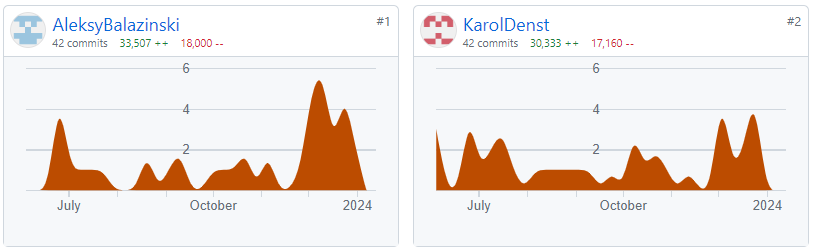
\includegraphics[width=0.8\textwidth]{chapters/introduction/work_distribution/resources/github_contributions.png}
    \caption{GitHub contributions (\url{https://github.com/Non-Euclidean-World/Hyper/graphs/contributors})}
    \label{fig:github_contributions}
\end{figure}

\begin{table}[!htb]
    \centering
    \begin{tabular}{|l|l|}
        \hline
        Task                                                          & Author            \\ \hline
        Implementation of the game logic                              & Both              \\
        Implementation of the graphics engine                         & Both              \\
        Implementation of terrain editing                             & Both              \\
        Implementation of the spherical geometry                      & Aleksy Bałaziński \\
        Implementation of the hyperbolic geometry                     & Aleksy Bałaziński \\
        Integration of the physics engine with the rest of the system & Aleksy Bałaziński \\
        Implementation of the terrain generation                      & Karol Denst       \\
        Implementation of the user interface (HUD \& Menu)            & Karol Denst       \\
        Implementation of character models and animations             & Karol Denst       \\
        \hline
    \end{tabular}
    \caption{Work distribution for the application}
    \label{tab:division_of_work_on_the_application}
\end{table}

\begin{table}[!htb]
    \centering
    \begin{tabular}{|l|l|l|}
        \hline
        Chapter                               & Section                                     & Author            \\ \hline
        \nameref{ch:introduction}             &                                             & Both              \\
        \nameref{sec:division_of_work}        &                                             & Both              \\
        \nameref{ch:functional_specification} &                                             & Both              \\
        \nameref{ch:theoretical_foundations}  & \nameref{sec:non_euclidean_geometry}        & Aleksy Bałaziński \\
        \nameref{ch:theoretical_foundations}  & \nameref{sec:theory_theory_marching_cubes}  & Karol Denst       \\
        \nameref{ch:theoretical_foundations}  & \nameref{sec:theory_theory_models}          & Karol Denst       \\
        \nameref{ch:theoretical_foundations}  & \nameref{sec:theory_theory_day_night_cycle} & Aleksy Bałaziński \\
        \nameref{ch:theoretical_foundations}  & \nameref{sec:theory_theory_lighting}        & Aleksy Bałaziński \\
        \nameref{ch:implementation}           & \nameref{sec:technologies_selection}        & Aleksy Bałaziński \\
        \nameref{ch:implementation}           & \nameref{sec:game_objects_management}       & Aleksy Bałaziński \\
        \nameref{ch:implementation}           & \nameref{sec:implementation_terrain}        & Karol Denst       \\
        \nameref{ch:implementation}           & \nameref{sec:chunk-worker}                  & Aleksy Bałaziński \\
        \nameref{ch:implementation}           & \nameref{sec:implementation_rendering}      & Aleksy Bałaziński \\
        \nameref{ch:implementation}           & \nameref{sec:two_dimensional_graphics}      & Karol Denst       \\
        \nameref{ch:testing}                  &                                             & Karol Denst       \\
        \nameref{ch:user_manual}              &                                             & Karol Denst       \\
        \nameref{ch:results}                  &                                             & Aleksy Bałaziński \\
        \nameref{ch:problems}                 &                                             & Karol Denst       \\
        \nameref{ch:improvements}             &                                             & Karol Denst       \\
        \hline
    \end{tabular}
    \caption{Work distribution for the document}
    \label{tab:division_of_work_on_the_document}
\end{table}
